% ==========================================
% Section 2: Errors in Data (Slides 6-7)
% ==========================================

% Slide 6: Errors in Data
\begin{frame}{خطاها در داده‌ها}
\begin{columns}[c]
  \begin{column}{0.58\textwidth}
    \begin{itemize}
      \item \textbf{منابع ایجاد خطا:}
      \begin{itemize}
        \item خرابی یا کالیبره نبودن حسگرها (\lr{Malfunctioning sensors})
        \item خطاهای ورود دستی داده‌ها (مانند جابجایی ارقام \lr{twisted digits})
        \item خطاهای ذخیره‌سازی و انتقال شبکه (\lr{Storage/transmission errors})
      \end{itemize}
      \vspace{0.3cm}
      \item \textbf{خطاهای انسانی:}
      \begin{itemize}
        \item پاسخ‌های تعمدی نامعتبر در پرسشنامه‌ها
        \item سوگیری در طرح سوالات یا برداشت کاربر
      \end{itemize}
    \end{itemize}
  \end{column}
  \begin{column}{0.40\textwidth}
    \centering
    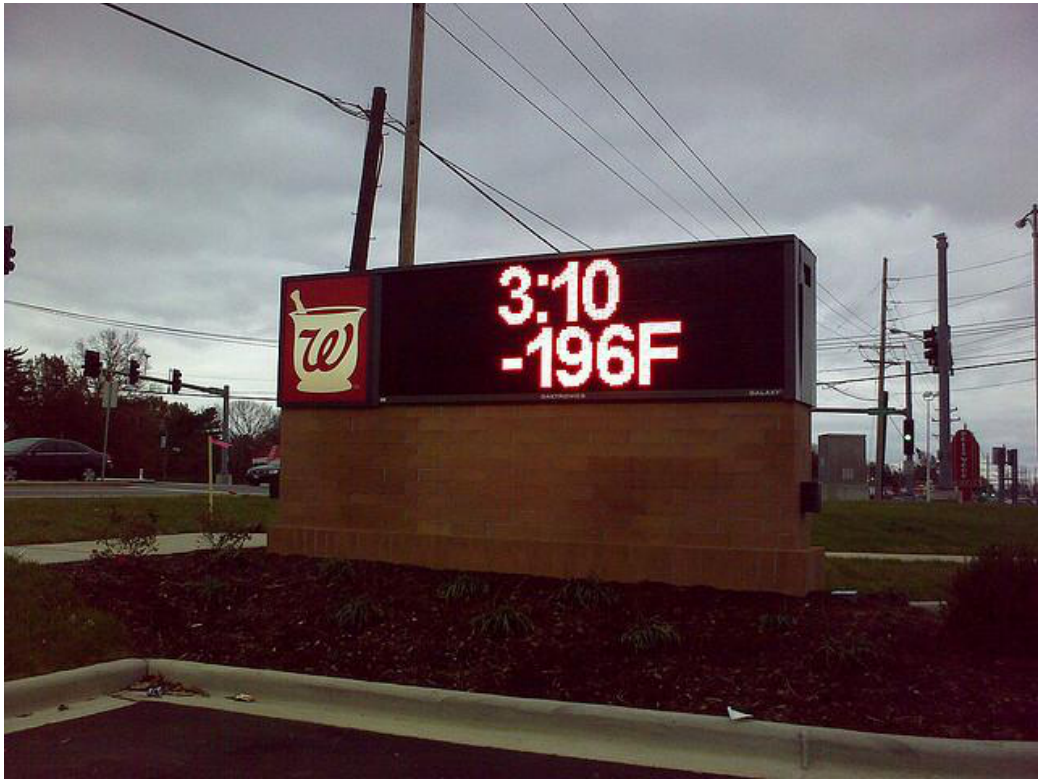
\includegraphics[width=\textwidth]{images/page_06_img_1.png}
  \end{column}
\end{columns}
\end{frame}

% Slide 7: Errors in Data - Remedies
\begin{frame}{خطاها در داده‌ها: راه‌حل‌ها}
\begin{itemize}
  \item \textbf{راه‌حل ساده و مستقیم:}
  \begin{itemize}
    \item حذف نقاط داده‌ای که خارج از یک بازه مجاز مشخص قرار دارند.
  \end{itemize}
  \vspace{0.2cm}
  \item \textbf{این کار نیازمند شناخت و دانش حوزه مسئله (\lr{Domain Knowledge}) است}
  \begin{itemize}
    \item حذف مقادیر دمای محیطی خارج از بازه $-30^\circ\text{C}$ تا $+50^\circ\text{C}$
    \item حذف مقادیر منفی برای متغیرهای مربوط به مدت‌زمان
    \item حذف تراکنش‌های خرید غیرعادی بالای ۱ میلیون یورو (احتمال تقلب یا ارقام ساختگی برای تست)
  \end{itemize}
  \vspace{0.2cm}
  \item \textbf{راه‌حل‌های پیشرفته‌تر:}
  \begin{itemize}
    \item شناسایی خودکار نمونه‌های داده مشکوک با استفاده از الگوریتم‌های تشخیص ناهنجاری (\lr{Anomaly / Outlier Detection})
    \item برازش توزیع‌های آماری بر متغیرها و بررسی فاصله نقاط از توزیع مورد انتظار
  \end{itemize}
\end{itemize}
\end{frame}
